\chapter{Technische Details vom DMX Protokoll}
\lhead{Kapitel 3: \emph{Technische Details vom DMX Protokoll}}

Ein DMX-Paket besteht aus verschiedenen Segmenten. Jedes Paket beginnt mit dem Halten von zwei Logiksignalen: Ein logisches Aus, gefolgt von einem logischen An. Das Logische An wird als Pause (\emph{Break}) im DMX-Protokoll definiert. Das logische Aus wird als \emph{MAB (Mark After Break)} definiert\cite[S.17]{DMX512-Protocol-Standard}. Das Pausesignal markiert den Anfang des Pakets. Nach dem Pausesignal folgen insgesamt bis zu 513 decodierte Bytes. Das erste Byte bestimmt den \emph{Startcode}. Der \emph{Startcode} beschreibt den Inhalt der nachfolgenden Bytes. Ein Standard DMX Paket fängt mit einem \emph{Startcode} gleich 0 an. Die restlichen Bytes im DMX-Protokoll werden für die bis zu 512 unterstützten Kanäle verwendet\cite[S.14]{DMX512-Protocol-Standard}. Das Pausesignal zusammen mit dem \emph{Startcode} wird als Reset Sequenz bezeichnet\cite[S.17]{DMX512-Protocol-Standard}.

\section{Verwendung des UART-Protokolls}

Die Decodierung aller Bytes erfolgen mithilfe der Verwendung des UART-Protokolls. UART ist ein serielles Datenprotokoll, bei dem die Bits nicht parallel über mehrere Kabel, sondern zeitlich nacheinander in der Leitung übertragen werden\cite[S.1]{UartStandard}.

Das UART-Protokoll verwendet eine zuvor beim Sender und Empfänger definierte Geschwindigkeit für die Datenübertragung \cite[S.2]{UartStandard}.  Das UART-Protokoll unterstützt optionale Start- und Stopbits, um die Stabilität zu erhöhen und die Datenintegrität zu prüfen\cite[S.2]{UartStandard}. Die Start- und Stopbits werden vor bzw. hinter dem gesendeten Byte verschickt. Das Startbit ist immer ein logische Aus, während die Stopbits aus einem logischen An bestehen\cite[S.2]{UartStandard}. Zusätzlich können Paritätsbits mitgesendet werden, um die Fehlertoleranz zu erhöhen\cite[S.2]{UartStandard}. Die Bits eines Bytes können beim UART-Protokoll in zwei verschiedenen Reihenfolgen gesendet werden: Entweder wird das
höchstwertige Bit (\emph{Most Significant Bit - MSB}) , oder das niedrigstwertige Bit (\emph{Least Significant Bit - LSB}) zuerst übertragen\cite[S.2]{UartStandard}. Sender und Empfänger müssen sich vor der Kommunikation über die Konfiguration abstimmen.

Das DMX-Protokoll basiert auf dem UART-Protokoll und verwendet ein Startbit, zwei Stopbits und fängt mit dem höchstwertigen Bit an. Die Bits werden mit einer Datenrate von $250 \frac{\SI{}{\kilo\bit}}{\SI{}{\s}}$ übertragen\cite[S.10]{DMX512-Protocol-Standard}.

In einem DMX-Paket werden mehrere Bytes zu einem Paket zusammengefasst. Ein Paket wird durch die Reset Sequenz markiert. Das Pause Signal in der Reset Sequenz ist jedoch nicht im UART-Protokoll definiert. Versucht man also, ein vollständiges DMX-Paket nur mit einem standardmäßigen UART-Empfänger zu empfangen, können nicht alle Teile des Signals erkannt werden, und das Paket kann nicht decodiert werden\cite[S.29]{RaspberryPiDmxInterface}.

\section{Aufbau des DMX-Pakets}

Im DMX Diagramm \ref{fig:DmxPacketDiagram} ist der Aufbau des DMX-Pakets dargestellt. Die einzelnen Elemente werden in den folgenden Unterabschnitten genauer erläutert.

\begin{figure}[H]
	\centering
	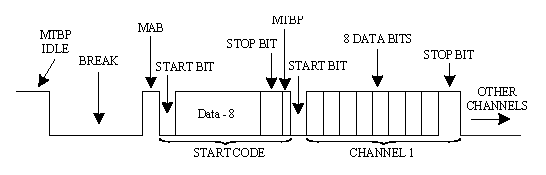
\includegraphics[width=0.8\linewidth]{Pictures/DmxTiming}
	\caption{DMX Paketdiagramm \cite[S.107]{DmxBiDerectionRdmDMX}}
	\label{fig:DmxPacketDiagram}
\end{figure}

Das Paket beginnt mit einem Pause Signal, welches für mindestens 92 µs gehalten werden muss \cite[S.18]{DMX512-Protocol-Standard}. Eine typische Länge beträgt 176 µs \cite[S.18]{DMX512-Protocol-Standard}. Nach dem Pause Signal folgt die \emph{Mark After Break (MAB)}. Die Mindestlänge des \emph{MAB} Signals beträgt 12 µs \cite[p.18]{DMX512-Protocol-Standard}.

Nach dem Pause Signal werden bis zu 513 Bytes übertragen. Der erste Byte ist der \emph{Startcode}. Das DMX-Paket beginnt mit einem \emph{Startcode} von 0. DMX wurde als unidirektionale Kommunikation entwickelt. Es gibt jedoch DMX-Erweiterungen wie z.B. RDM, die eine bidirektionale Kommunikation zwischen DMX Konsole und Leuchte ermöglichen \cite[p.23]{DMX512-Protocol-Standard}. Ein RDM Signal kann beispielsweise einen anderen \emph{Startcode} enthalten. Das Pause- und \emph{MAB} Signal zusammen mit dem \emph{Startcode} wird als Reset Sequenz bezeichnet. Die  Reset Sequenz wird benötigt, um den Anfang eines Datenpakets zu beschreiben und die verschiedenen Datenpakete voneinander zu unterscheiden.

Nach der Reset-Sequenz folgen die Kanäle des DMX-Protokolls. Es können zwischen 1 und 512 Kanäle übertragen werden. Jeder Kanal wird von einem Byte repräsentiert \cite[p.10]{DMX512-Protocol-Standard}. Daher kann jeder Kanal einen Wert zwischen 0 und 255 annehmen.

\section{Zeitdiagramm}

Im DMX Paket Diagramm \ref{fig:DmxTimingFrame} ist die  genaue Struktur des DMX Protokolls veranschaulicht.

\begin{figure}[H]
	\centering
	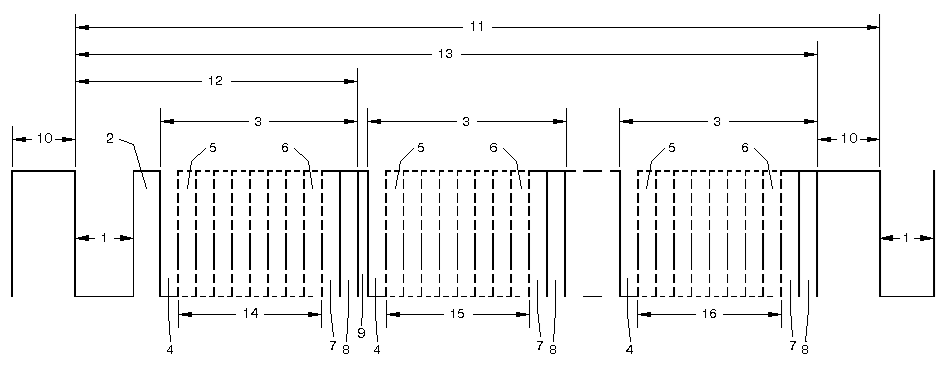
\includegraphics[width=\linewidth]{Pictures/DmxTimingFrame}
	\resizebox{\textwidth}{!}{ %
		\begin{minipage}{0.5 \linewidth}
			\centering
			\begin{tabular}{ r l}
				1: 	& Space for Break\\
				2:	& Mark after Break (MAB)\\
				3:	& Slot Time\\
				4:	& START Bit\\
				5:	& Least Significant Data Bit\\
				6:	& Most Significant Data Bit\\
				7, 8:	& Stop Bit\\
				9:	& Mark Time between slots\\
			\end{tabular}
		\end{minipage}\hfill
		\begin{minipage}{0.5 \linewidth}
			\begin{tabular}{ r l}
				10:	& Mark before break (MBB)\\
				11:	& Break to break Time\\
				12:	& Reset Sequence (Break, MAB, Start
				Code)\\
				13:	& DMX512 Packet\\
				14:	& Start code (Slot 0 Data)\\
				15:	& Slot 1 Data\\
				16:	& Slot nnn Data (Maximum 512)\\
			\end{tabular}
		\end{minipage}
	}
	
	\caption{DMX Paket \cite[S.17]{DMX512-Protocol-Standard}}
	\label{fig:DmxTimingFrame}
\end{figure}

Die Zeitabstände, die im DMX-Protokoll verwendet werden, sind in der Tabelle \ref{tab:timingChart} aufgeschlüsselt. Die Zeitabstände sind detailliert aufgeführt und zeigen die minimalen, typischen und maximal erlaubten Zeitabstände innerhalb des DMX Standards.

\begin{table}[H]
	\centering
	\resizebox{\textwidth}{!}{ %
		\begin{tabular}{ |c|c|c|c|c|c| } 
			\hline
			Nr. & Beschreibung & Min & Typ & Max & Einheit \\
			\hline
			-  & Bit Übertragungsrate	&	245 	& 250 	& 255 	& $\frac{\SI{}{\kilo\bit}}{\SI{}{\s}}$ \\
			-  & Bitlänge	&	3.92	&  4	& 4.08 	& µs\\
			-  & minimale Aktualisierungszeit bei 513 Bytes 	& – & 22.7	& – & ms\\
			-  & maximale Aktualisierungsrate bei 513 Bytes & – & 44	& – & $\frac{\SI{}{Aktualisierungen}}{\SI{}{\s}}$\\
			1  & Raum für Pause 	& 92 & 176 & – &  µs\\
			2  & Mark Break (MAB)		& 12 $|$  – & – & – $|$  $<$ 1.00 & µs $|$  s \\
			9  & Markierungszeit zwischen Bytes 	& 0  & – & $<$ 1.00 & s\\
			10 & Mark Before BREAK (MBB)	& 0  & – & $<$ 1.00 & s\\
			11 & Pause zu Pause Zeit & 1204 $|$ – & – & – $|$ 1.00   & µs $|$ s \\
			13 & DMX512 Paket & 1204 $|$ – & – & – $|$ 1.00 & µs $|$ s \\
			\hline
	\end{tabular}}
	\caption{Zeitdiagramm \cite[S.18]{DMX512-Protocol-Standard}}
	\label{tab:timingChart}
\end{table}

Es ist wichtig, diese Werte zu berücksichtigen, um sicherzustellen, dass die DMX Übertragung korrekt empfangen werden kann. Wird dies nicht berücksichtigt, kann es passieren, dass einige Geräte in der DMX-Kette die Daten nicht decodieren können.


Zusammenfassend basiert das DMX-Protokoll auf dem UART-Protokoll und verwendet eine Reihe von Zeitabständen, welche die Kommunikation zwischen DMX Geräten definiert. Es ist entscheidend, diese Elemente und ihre jeweiligen Zeitanforderungen zu verstehen, um ein korrekt funktionierendes DMX-System aufzubauen und zu betreiben. Diese Zeitabstände werden in dem gebauten DMX Analysator auch genauer untersucht.

